\subsection{Localizing brain sources responding to glitches in VR}
With an across-participants average classification accuracy of ~78 percent the linear discrimination between mismatch and match trials exceeded chance level at \~56 percent, $t_{18} = 42.1, P = 0$. In the fourth (200-250 ms) and sixth (300-350 ms) time window post event the control signal, that is channel activity weighted by classification weights, showed a clear separation between classes, see \ref{lda} B and C.

% the ttest against simulatedchance is kinda weird
% check ~ sign in latex
% is lda control signal well explained or is it over irrelevant for the paper

\begin{figure}[h]
  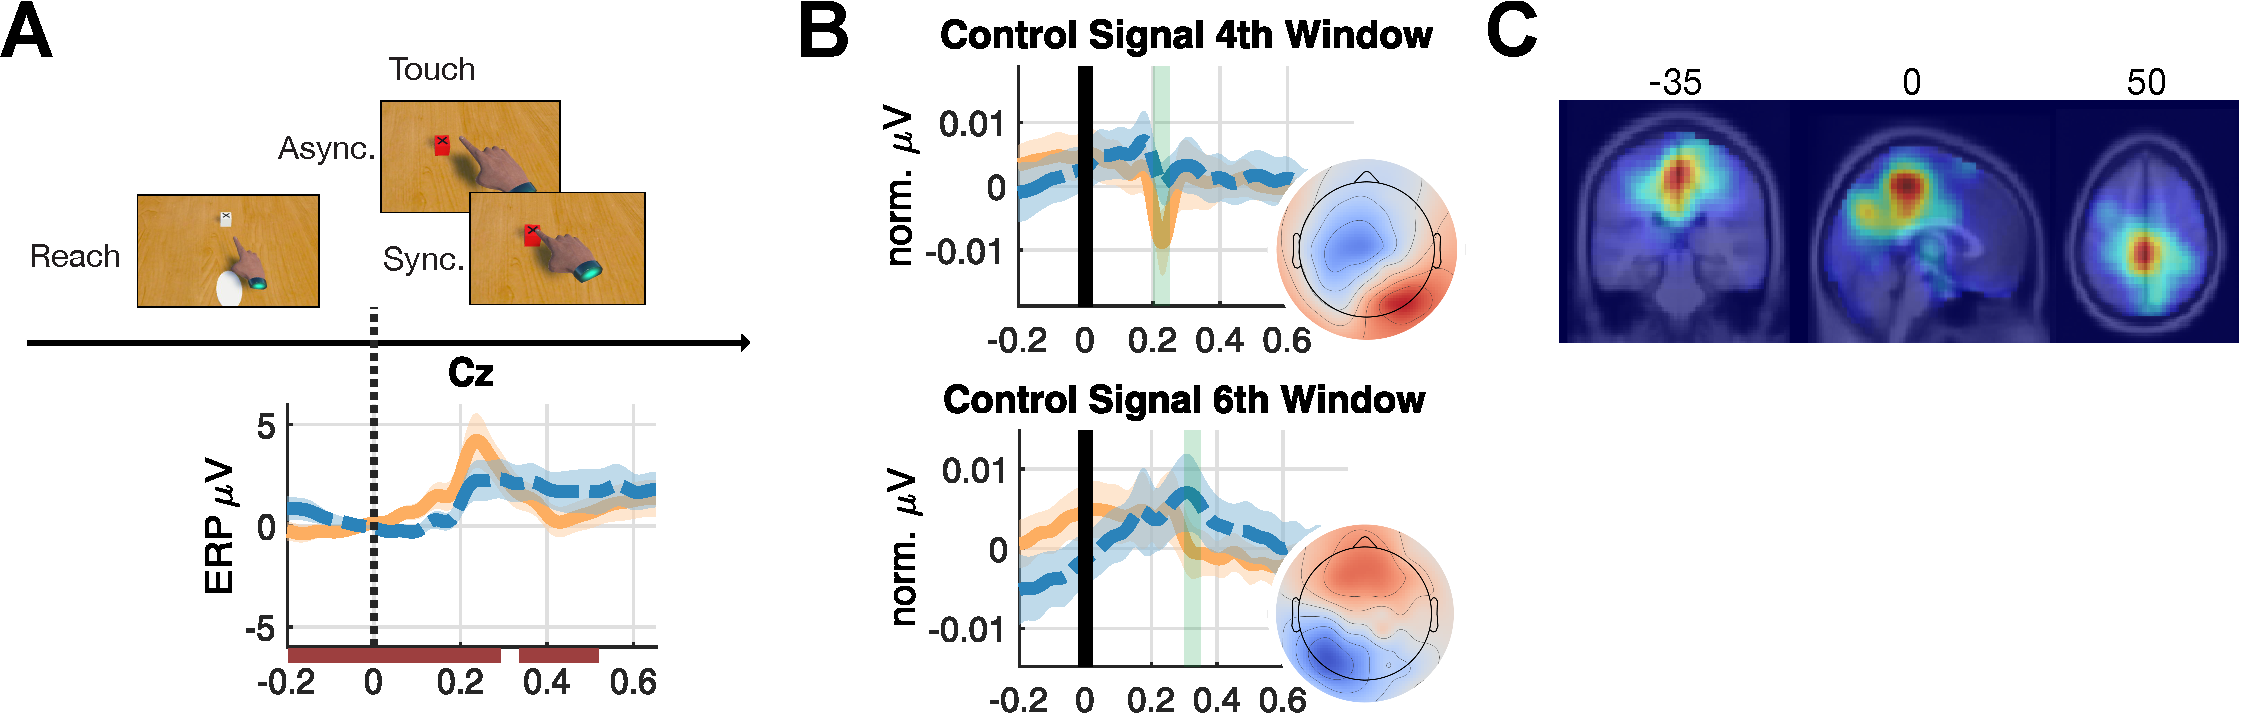
\includegraphics[width=\textwidth]{figures/fig2_discrimination_short.pdf}
  \caption{\textbf{A} An LDA classifier was trained on eight windowed means of 50 ms size from 50 to 450 ms following object selection. Two classes of synchronous and asynchronous trials were labeled for training and cross-validation. Bottom, grand-average ERP of projected source mixture at electrode Cz with significant class differences marked. \textbf{B} Grand-average ERP projected through sources of focus in the 4th and 6th time windows respectively with scalp map of control signal activity. \textbf{C} Localization of focused sources on average across all time windows used to determine seed for region of interest clustering of independent components.}
  \label{lda}
\end{figure}
With the goal to employ the trained BCI classifier for neuroscientific inquiry, we investigated which EEG effective sources contributed maximally to the classification. This source reconstruction serves two purposes: (1) Asserting that the classifier does not rely primarily on artifact EEG sources, and (2) gain additional information about the contributing brain regions to allow neuroscientific interpretations.

% TODO
% [] add link back to intro about usefulness for application in neural interface tech

Across all time windows, a prominent source location contributing maximally to the classification was identified in the brain at a central-parietal location (MNI X = 0, Y = -35, Z = 50).